\documentclass[fullscreen=true, bookmarks=true, hyperref={pdfencoding=unicode}]{beamer}

\usepackage[utf8]{inputenc}                                % Кодировка
\usepackage[english,russian]{babel}                        % Переносы
\usepackage{xcolor}                                        % Работа с цветом
\usepackage{amsmath,amssymb,amsfonts}                      % Символы АМО
\usepackage{graphicx}                                      % Графика
\usepackage[labelsep=period]{caption}                      % Разделитель в подписях к рисункам и таблицам
\usepackage{hhline}                                        % Для верстки линий в таблицах
\usepackage[upright]{fourier}
\usepackage{verbatim}
\usepackage{tikz}                                          % Для простых рисунков в документе
\usetikzlibrary{matrix,arrows,decorations.pathmorphing,shapes.geometric}
\usepackage{fancybox}                                      % Пакет для отрисовки рамок
\usepackage{verbatim}                                      % Для вставки кода в презентацию
% \usepackage{animate}                                       % Для вставки видео в презентацию
\usepackage{xmpmulti}                                      % Для вставки gif в презентацию
\usepackage{multirow}
% \usepackage{media9}                                        % To include youtube video
\usepackage{circuitikz}

\usetikzlibrary{arrows,snakes,backgrounds}                 % Для отрисовки стрелок

\graphicspath{{../images/}}                                % Путь до рисунков
\setbeamertemplate{caption}[numbered]                      % Включение нумерации рисунков

\definecolor{links}{HTML}{2A1B81}                          % blue for url links
\hypersetup{colorlinks,linkcolor=,urlcolor=links}          % nothing for others

\usetheme{Malmoe}
\usecolortheme{seahorse}

% l' unite
\newcommand{\myunit}{1 cm}
\tikzset{
    node style sp/.style={draw,circle,minimum size=\myunit},
    node style ge/.style={circle,minimum size=\myunit},
    arrow style mul/.style={draw,sloped,midway,fill=white},
    arrow style plus/.style={midway,sloped,fill=white},
}

% \setbeameroption{show notes}
\setbeameroption{hide notes}

\title{Lecture 1. Intro, systems of linear equations, matrices}
\author{Aleks Avdiushenko}
\institute{Neapolis University Paphos}
\date{May 10, 2023}
\titlegraphic{
\includegraphics[keepaspectratio,width=0.25\textwidth]{nup_logo.png}}

\begin{document}
%\unitlength=2mm

% выводим заглавие
\begin{frame}
\transdissolve[duration=0.2]
\titlepage
\end{frame}

\begin{frame}
  \frametitle{First data scientist}
  
  \pause
  \begin{center}
    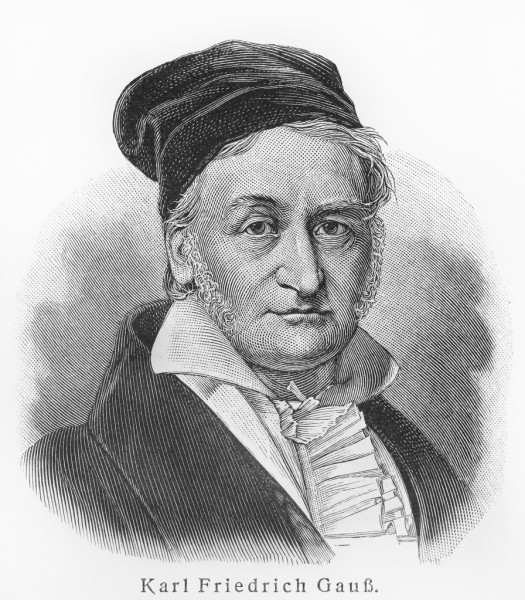
\includegraphics[keepaspectratio, width=.4\paperwidth]{carl-gauss.jpg}
  
    Mathematician, mechanic, physicist, astronomer      
  \end{center}

  \pause 
  At the age of 24 in 1801, he predicted where to look for the dwarf planet Ceres, 
  hidden behind the Sun

  \note{Who was the first data scientist? Then in the 18-th century there was no machine learning 
  and computers, but people had roughly the same problems as we have. 
  For example, where did the minor planet Ceres disappear from the sky? 
  On 1 January 1801, Italian astronomer Giuseppe Piazzi discovered the dwarf planet Ceres.
  Piazzi could track Ceres for only somewhat more than a month, 
  following it for three degrees across the night sky. Then it disappeared temporarily 
  behind the glare of the Sun. Several months later, when Ceres should have reappeared, 
  Piazzi could not locate it: the mathematical tools of the time were not able to extrapolate 
  a position from such a small amount of data — three degrees represent less than 1\% 
  of the total orbit. Gauss heard about the problem and tackled it. 
  After three months of intense work, he predicted a position for Ceres in December 1801 — 
  just about a year after its first sighting.
  }  
\end{frame}


\begin{frame}
  \frametitle{Course program}
  
  \pause
  Linear algebra
  {\scriptsize
  \begin{itemize}
      \item \textbf{Systems of linear equations, matrices}, operations, block operations, 
      reversibility and non-degeneracy
      \item \textbf{Determinants} (3 approaches), oriented volumes, explicit inverse matrix formulas, 
      characteristic polynomial, polynomial calculus in matrices, spectrum, Hamilton-Cayley theorem
      \item \textbf{Vector spaces} and subspaces, dimensions, matrix ranks: row rank, column rank, 
      factorial rank, tensor rank, minor rank. Properties of ranks and inequalities on ranks
      \item \textbf{Linear mappings} and their matrix description, change of coordinates. 
      The image and the kernel, their geometric meaning, connection to the dimension. 
      Linear operator invariants: trace, determinant, characteristic polynomial. 
      Eigenvalues and vectors, connection with the spectrum
      A note about complex numbers. Diagonalizability and related matrix expansions
      \item \textbf{Bilinear forms}. Quadratic forms and symmetric bilinear forms
      Signature, its geometric meaning, methods for determining the signature. 
      Relationship with LU-decomposition. Dot products, angles and distances. 
      Orthogonalization and QR-decomposition. Linear manifolds and linear classifiers, margins
      \item \textbf{Operators in Euclidean spaces}. Motions and orthogonal matrices and their classification. 
      Self-adjoint operators and symmetric matrices, their diagonalizability. 
      Singular value decomposition (SVD). Finding SVD
  \end{itemize}
  }
\end{frame}


\begin{frame}
  Probability theory
  {\scriptsize
  \begin{itemize}
    \item \textbf{Probability space}, random events, how to understand them. 
    Probability (measure) and conditional probability, independence of events, geometric meaning. 
    Bayes formulas and full probability
    \item \textbf{Random variables}, how to understand them. Distribution functions, probabilities (measures) 
    on the line and how to set them. Classes of distributions, examples of discrete and 
    continuous distributions. Joint distribution. Characteristics of random variables: 
    mathematical expectation, variance, moments, median (in a good case). 
    Normal or Gaussian distribution
    \item \textbf{Random vector} or multidimensional random variable, how to understand and set them. 
    Classes of distributions, examples of discrete and continuous distributions. 
    Recovery of distributions of coordinates. Mathematical expectation and covariance matrix. 
    Independence of random variables. Properties of mathematical expectation 
    and dispersion for independent random variables
    \item \textbf{Conditional mathematical expectations and probabilities}. Bayes formulas and 
    full probability for the continuous case. 
    Distribution of the sum of independent random variables and convolution of densities. 
    Multivariate Gaussian distribution
  \end{itemize}
  }

\end{frame}


\begin{frame}[t]
  Mathematical statistics
  {\scriptsize
  \begin{itemize}
    \item \textbf{The basic model of mathematical statistics} (how to relate the formalism of 
    probability theory to sample measurements). Estimates and their properties. 
    Why convergence and limit theorems are needed. Types of convergences and the relationship between them. 
    Laws of large numbers and Chebyshev's inequality. 
    Sample mean and sample variance, sample covariance matrix, correlation coefficient. 
    Maximum likelihood method. PCA and SVD. Central limit theorem and the Berry-Essen inequality
    \item \textbf{Generating a random sample}. Probability integral transformation. Direct and non-direct methods. 
    Accept-Reject algorithm. MCMC algorithms, Metropolis Algorithm
    \item \textbf{Hypothesis testing}. Formal problem of hypothesis testing. Differences of parametric and non-parametric 
    tests. Confidence intervals. Examples of hypotheses and tests 
    \item \textbf{Parametric and non-parametric tests}. Type-I, Type-II errors, p-value. Choosing the methods. Student-T and U-Mann-Whitney. 
    Normality tests, Shapiro-Wilk W-Test
    \item \textbf{ANOVA family}. Formal problem. ANOVA assumptions. Theoretical basis of one way ANOVA. Two-way ANOVA. 
    N-way ANOVA, non-parametric ANOVA, ANCOVA
    \item \textbf{Bootstrap}. Theory and practice
    \item \textbf{Introduction in Bayesian Statistics}. Theory and practice
  \end{itemize}
  }
\end{frame}


\begin{frame}[t]
  \frametitle{Homework Assignments and Grading Rules}

  {\scriptsize
  \begin{itemize}
    \item The course consists of 13 classes. There will be a homework assignment 
  for each class. The deadline for each homework assignment is 10 days 
  from the date of publication (the deadline will be indicated 
  in the assignment). 
  \item If an assignment is submitted after the deadline, 
  the final grade is calculated using the 
  formula $O_{\text{final}} = 0.7^t O_{\text{hw}}$, 
  where $t$ is the time after the deadline in days without rounding, 
  $O_{\text{hw}}$ is the grade for the homework assignment 
  if it had been submitted on time, and 
  $O_{\text{final}}$ is the grade awarded for the late homework assignment.
  
  \item Homework assignments must be submitted in written form 
  (handwritten or using \LaTeX, virtual boards are also acceptable). 
  The work should be submitted as a single multi-page PDF file 
  (you can use the \texttt{notebloc} app on your mobile phone, as it does 
  a good job of whitening the background and produces photos 
  of acceptable size). 
  All pages must be vertically oriented and in sequential order. 
  Please make sure to adhere to this requirement. We would be very grateful for your cooperation.
  
  \item The rules for determining the final grade will be announced later, 
  but by default, it is assumed that all 13 homework assignments 
  must be completed. The threshold value for passing the course 
  will be announced later.

  \item As a midterm there will be a offline written test with tasks 
  similar to homework assignments.
  \end{itemize}
  }
\end{frame}


\begin{frame}{Why do you need linear algebra?}
  Consider Kirchhoff's Circuit Laws for example.
  \begin{itemize}
  \item Two fundamental laws for electric circuits:
    \begin{enumerate}
      \item Kirchhoff's Current Law (KCL)
      \item Kirchhoff's Voltage Law (KVL)
    \end{enumerate}
  \pause\item KCL: the sum of currents entering a node equals the sum of currents leaving the node
  \pause\item KVL: the sum of the voltage differences (potential drops) around any closed loop or mesh in a network is zero
  \pause\item Applying KCL and KVL to a circuit leads to a system of linear algebraic equations
  \end{itemize}  
\end{frame}  


\begin{frame}
\begin{block}{Example Circuit}
  \vspace{0.2cm}
    \begin{circuitikz}
    \draw (0,0) to[V, l=$V$] (0,2) -- (2,2) to[R, l=$R_1$] (2,0) -- (0,0);
    \draw (2,2) -- (4,2) to[R, l=$R_2$] (4,0) -- (2,0);
    \draw (4,2) -- (6,2) to[R, l=$R_3$] (6,0) -- (4,0);
    \draw (6,2) -- (8,2) to[R, l=$R_4$] (8,0) -- (6,0);
    
    \node[ground] at (0,0) {};
    \node at (1,0) [below] {$I_1$};
    \node at (3,0) [below] {$I_2$};
    \node at (5,0) [below] {$I_3$};
    \node at (7,0) [below] {$I_4$};
  \end{circuitikz}  
\end{block}  
\centering
$I_1, \dots, I_4 \in \mathbb{R}$ are variables, $R_i$ — resistances

\pause
\begin{align*}
  R_1 I_1 - R_1 I_2 &= V \\
  R_2 I_2 - R_2 I_3 &= V \\
  R_3 I_3 - R_3 I_4 &= V \\
  R_4 I_4 &= V 
  \end{align*}
\end{frame}


\begin{frame}
  \frametitle{System of linear equations in general form}
  $x_1, \dots, x_n \in \mathbb{R}$ are variables
  $$\left\{\begin{matrix}
    a_{11}x_1 & +a_{12}x_2 & +\dots &  +a_{1n} x_n & = & b_1 \\
    a_{21}x_1 & +a_{22}x_2 & +\dots &  +a_{2n} x_n & = & b_2 \\
              &            & \vdots &              &   & \vdots\\
    a_{n1}x_1 & +a_{n2}x_2 & +\dots &  +a_{nn} x_n & = & b_n
  \end{matrix}\right. \qquad
  a_{ij}, b_i \in \mathbb{R}
  $$

  \pause
  We can easily check by substitution, if $(c_1, \dots, c_n)$ is solution.

  \pause
  \vspace{0.5cm}
  \begin{block}{Question 1}
    But how to find all solutions effectively?
  \end{block} 

  \pause
  \vspace{0.5cm}
  We can \textbf{transform} the system to a form where 
  all solutions become easy to find:
  $S_1 \rightarrow S_2 \rightarrow \dots \rightarrow S_k$
\end{frame}


\begin{frame}
  \frametitle{Elementary Row Transformations}
  \note{Row transformations are performed only on the basis 
  of a few sets of rules. An individual cannot perform 
  any other kind of row operation apart from the below-stated rules. 
  There are three kinds of elementary row transformations.} 

  Three kinds of elementary row transformations
  \begin{itemize}
    \pause\item Interchanging the rows: 
    the entire row $R_i$ is swapped with another row $R_j$
    \pause\item Scaling the entire row with a non zero number: 
    $R_i \rightarrow \lambda R_i$
    \pause\item Add one row to another row multiplied by a non zero number: 
    $R_i \rightarrow R_i + \lambda R_j$ 
\end{itemize}
\end{frame}


\begin{frame}
  \frametitle{Gauss-Jordan elimination algorithm}
  \framesubtitle{row reduction}
  A matrix can always be transformed into an \textbf{upper triangular matrix}
  using elementary row transformations.

  $$\left[\begin{matrix}
    1 & -2 & 1  & 0 \\
    2 &  1 & -3 & 5 \\
   -4 &  7 & -1 & 1 \\
  \end{matrix}\right]
  \quad \rightarrow \quad
  \left[\begin{matrix}
    1 & -2 & 1 & 0 \\
    \cline{1-1}
    0 & \multicolumn{1}{|c}{-1} & 3 & 1  \\
    \cline{2-2}
    0 & 0 & \multicolumn{1}{|c}{10} & 10 \\
  \end{matrix}\right]$$

  \vspace{1cm}
  In genral rectangular case it is called row echelon form.
\end{frame}


\begin{frame}
  \frametitle{Demo Video}
  
  \href{https://www.youtube.com/watch?v=xivbwsMyorU}{Youtube link}

\end{frame}


\begin{frame}
  \frametitle{\textbf{Principal} and free variables}

  \begin{eqnarray*}
    \begin{matrix} \boldsymbol{x}_1 &  & \boldsymbol{x}_3 &  & \end{matrix} \quad\ \\
  \left[\begin{matrix}
    1 & 1 & 0 & 2 & \multicolumn{1}{|c}{3} \\
    \cline{1-2}
    0 & 0 & \multicolumn{1}{|c}{1} & 5 & \multicolumn{1}{|c}{4} \\
    \cline{3-4}
  \end{matrix}\right] \\
  \begin{matrix} & x_2 &  & x_4 &  \end{matrix} \quad
  \end{eqnarray*} 

  \pause

  \vspace{0.5cm}
  \begin{block}{Question 2}
    How many principal variables is for different values $x$?

    \begin{equation*}
      \left[\begin{matrix}
        x & 1 & 1 & 1 & \multicolumn{1}{|c}{0} \\
        1 & x & \dots & 1 & \multicolumn{1}{|c}{0} \\
        1 & \dots & \ddots & 1 & \multicolumn{1}{|c}{0} \\
        1 & 1 & 1 & x & \multicolumn{1}{|c}{0} \\
        \end{matrix}\right]
    \end{equation*}
  \end{block} 

\end{frame}


\begin{frame}
  \frametitle{Solution scheme and answers}

  \begin{block}{Hint!}
    Try to add all rows to the first.
  \end{block}
    
  \pause\vspace{1cm}
  \begin{center}    
  \begin{tikzpicture}[every node/.style={ellipse,draw}, 
    level 1/.style={sibling distance=50mm}, 
    level 2/.style={sibling distance=25mm}]
  \node{$x + n - 1 = 0 ?$}
    child{node{$x=1?$}
      child{node{n}}
      child{node{1}}
    }
    child{node{n-1}
    };
  \end{tikzpicture}
  \end{center}
    
\end{frame}

\begin{frame}
  \frametitle{Homogeneous system}

  Right hand side equals zero:

  \begin{equation*}
    \underbrace{
        \left[\begin{matrix}
          \quad & R_1  & \quad & \multicolumn{1}{|c}{0} \\
          & R_2  &   & \multicolumn{1}{|c}{0} \\
          & \vdots &   & \multicolumn{1}{|c}{0} \\
          & R_m  &   & \multicolumn{1}{|c}{0} \\
        \end{matrix}\right]
    }_{n+1}
  \end{equation*}

  \pause
  \begin{block}{Fact}
    $n>m \Rightarrow \exists $ nontrivial solution 
  \end{block}
\end{frame}


\begin{frame}
  \frametitle{Operations on matrices}
  $M_{mn}(\mathbb{R}):$
  $$\left[\begin{matrix}
    a_{11} & a_{12} & \dots &  a_{1n} \\
    a_{21} & a_{22} & \dots &  a_{2n} \\
           &        & \vdots &        \\
    a_{m1} & a_{m2} & \dots &  a_{mn} 
  \end{matrix}\right] \qquad a_{ij} \in \mathbb{R}
  $$

  Operations
  \begin{enumerate}
    \item Addition and substraction — component wise
    \item Multiplication by a number — component wise
  \end{enumerate}

\end{frame}


\begin{frame}{3. Matrix multiplication}
  Let $A$ be an $m \times n$ matrix and $B$ be an $n \times p$ matrix. 
  The product $C = AB$ of $A$ and $B$ has $m \times p$ shape and is given by:
  {\small
  \[
  \underbrace{
    \begin{bmatrix}
    a_{11} & a_{12} & \dots & a_{1n} \\
    a_{21} & a_{22} & \dots & a_{2n} \\
    \vdots & \vdots & \ddots & \vdots \\
    a_{m1} & a_{m2} & \dots & a_{mn}
    \end{bmatrix}
  }_{m \times n}
  \underbrace{
    \begin{bmatrix}
    b_{11} & b_{12} & \dots & b_{1p} \\
    b_{21} & b_{22} & \dots & b_{2p} \\
    \vdots & \vdots & \ddots & \vdots \\
    b_{n1} & b_{n2} & \dots & b_{np}
    \end{bmatrix}
  }_{n \times p}
    =
  \underbrace{
      \begin{bmatrix}
    c_{11} & c_{12} & \dots & c_{1p} \\
    c_{21} & c_{22} & \dots & c_{2p} \\
    \vdots & \vdots & \ddots & \vdots \\
    c_{m1} & c_{m2} & \dots & c_{mp}
    \end{bmatrix}
  }_{m \times p}
    \]
  }
  where $$c_{ij} = \sum\limits_{k=1}^n a_{ik}b_{kj}$$ 
  for $i=1,\dots,m$ and $j=1,\dots,p$
\end{frame}


\begin{frame}{First example}
  \newcommand{\sidelen}{3cm}
  \newcommand{\shift}{0.5cm}
  \begin{tikzpicture}
    \coordinate (A) at (0, 0);
    \coordinate (C) at (-\sidelen, 0);
    \coordinate (D1) at (0, \sidelen);
    \coordinate (D2) at (-\sidelen, \sidelen);
    \coordinate [label={$\begin{matrix}
      0 & 1 &  & \\
       & \ddots & \ddots & \\
       &  & \ddots & 1 \\
       &  &  & 0 \\
      \end{matrix}$}] (Am) at (-\sidelen/2, \shift/2);

    \coordinate (Ar) at (\sidelen+\shift, 0);
    \coordinate (Cr) at (\shift, 0);  
    \coordinate (D1r) at (\sidelen+\shift, \sidelen);
    \coordinate (D2r) at (\shift, \sidelen);
    \coordinate [label={$A$}] (Arm) at (\sidelen/2+\shift, \sidelen/2-\shift/2);
    
    \coordinate (Arr) at (2*\sidelen+2*\shift, 0);
    \coordinate (Crr) at (\sidelen+2*\shift, 0);
    \coordinate (D1rr) at (2*\sidelen+2*\shift, \sidelen);
    \coordinate (D2rr) at (\sidelen+2*\shift, \sidelen);
    
    \draw [thick] (C) -- node [below left]  {} (A)
                      -- node [below left]  {} (D1)
                      -- node [above] {$n$} (D2)
                      -- node [left] {$m$} (C);

    \draw [thick] (Cr) -- node [below left]  {} (Ar)
                       -- node [below left]  {} (D1r)
                       -- node [above] {$n$} (D2r)
                       -- node [left] {$n$} (Cr);

    \draw [thick] (Crr) -- node [below left]  {} (Arr)
                       -- node [right]  {} (D1rr)
                       -- node [above] {$n$} (D2rr)
                       -- node [left] {$=$} (Crr);
    \pause
    \coordinate [label={$ \begin{matrix}
       & & & \\
       & & & \\
       & & & \\
      0 & \dots & \dots & 0 \\
      \end{matrix}$}] (Arrm) at (3*\sidelen/2+2*\shift, -0.3*\shift);
      \draw [dashed, red] (\sidelen+2*\shift, \shift) -- ++ (0, \sidelen)
      -- ++  (\sidelen, 0) -- node [right] {$m$} ++ (0, -\sidelen) -- ++ (-\sidelen, 0);
      \coordinate [label={$A$}] (Arrm) at (3*\sidelen/2+2*\shift, \sidelen/2);
  \end{tikzpicture}
\end{frame}


\begin{frame}{Second example}
  \newcommand{\sidelen}{3cm}
  \newcommand{\shift}{0.5cm}
  \begin{tikzpicture}
    \coordinate (A) at (0, 0);
    \coordinate (C) at (-\sidelen, 0);
    \coordinate (D1) at (0, \sidelen);
    \coordinate (D2) at (-\sidelen, \sidelen);
    \coordinate [label={$A$}] (Am) at (-\sidelen/2, \sidelen/2-\shift/2);

    \coordinate (Ar) at (\sidelen+\shift, 0);
    \coordinate (Cr) at (\shift, 0);  
    \coordinate (D1r) at (\sidelen+\shift, \sidelen);
    \coordinate (D2r) at (\shift, \sidelen);
    \coordinate [label={$\begin{matrix}
      0 & 1 &  & \\
       & \ddots & \ddots & \\
       &  & \ddots & 1 \\
       &  &  & 0 \\
      \end{matrix}$}] (Arm) at (\sidelen/2+\shift, \shift/2);
    
    \coordinate (Arr) at (2*\sidelen+2*\shift, 0);
    \coordinate (Crr) at (\sidelen+2*\shift, 0);
    \coordinate (D1rr) at (2*\sidelen+2*\shift, \sidelen);
    \coordinate (D2rr) at (\sidelen+2*\shift, \sidelen);
    
    \draw [thick] (C) -- node [below left]  {} (A)
                      -- node [below left]  {} (D1)
                      -- node [above] {$n$} (D2)
                      -- node [left] {$m$} (C);

    \draw [thick] (Cr) -- node [below left]  {} (Ar)
                       -- node [below left]  {} (D1r)
                       -- node [above] {$n$} (D2r)
                       -- node [left] {$n$} (Cr);

    \draw [thick] (Crr) -- node [below left]  {} (Arr)
                       -- node [right]  {} (D1rr)
                       -- node [above right] {$n$} (D2rr)
                       -- node [left] {$=$} (Crr);
    \pause
    \coordinate [label={$\quad\quad \begin{matrix}
      0 & & & \\
      \vdots & & & \\
      \vdots & & & \\
      0 & & & \\
      \end{matrix} \quad\ A$}] (Arrm) at (3*\sidelen/2+\shift, \shift/2);
      \draw [dashed, red] (\sidelen+3.5*\shift, 0) -- ++ (0, \sidelen)
      -- ++  (\sidelen, 0) -- node [right] {$m$} ++ (0, -\sidelen) -- ++ (-\sidelen, 0);
  \end{tikzpicture}

\end{frame}


\begin{frame}{Mnemonic rule}
  Multiplication from the \textbf{right} side operates on \textbf{columns}, 
  
  and on the \textbf{left} on \textbf{rows}.

  \pause
  \begin{block}{Question 3}
    What if we multiply on the diagonal matrix?

    \begin{equation*}
      \left[\begin{matrix}
        \lambda_1 & 0 & 0 & 0  \\
        0 & \lambda_2 & 0 & 0  \\
        0 & 0 & \lambda_3 & 0  \\
        0 & 0 & 0 & \lambda_4  \\
        \end{matrix}\right]
    \end{equation*}
  \end{block} 

\end{frame}


\begin{frame}{Properties of matrix operations}

  \begin{enumerate}
    \item $(AB)C = A(BC)$ — associativity
    \item $A(B+C) = AB+AC$ — distributivity
    \item $(A+B)C = AC+BC$
    \pause 
    \item $AB \neq BA$ (and even it is not possible sometimes)
    \pause 
    \item Zero divisors: $AB = 0$, when $A \neq 0$ and $B \neq 0$
    \item Nilpotents: $A \neq 0$, but $A^k = 0$
    \pause 
    \item $Ax=b$ — matrix form of system of linear equations
  \end{enumerate}

  \pause
  \begin{block}{Question 4}
    For which matrices A the equalty $A\Lambda = \Lambda A$ is true, where

  \begin{equation*}
    \Lambda = \left[\begin{matrix}
      \lambda_1 & 0 & 0 & 0  \\
      0 & \lambda_2 & 0 & 0  \\
      0 & 0 & \ddots & 0     \\
      0 & 0 & 0 & \lambda_k  \\
      \end{matrix}\right]
  \end{equation*}
  \end{block} 
\end{frame}


\begin{frame}{Block formula}
  Blocks as «numbers»:
  \vspace{1cm}

  \newcommand{\sidelen}{3cm}
  \newcommand{\shift}{0.25cm}
  \begin{tikzpicture}
    \draw (0, 0) -- ++ (0, \sidelen) -- ++  (\sidelen, 0) 
    -- ++ (0, -\sidelen) -- ++ (-\sidelen, 0);
    \draw (0, \sidelen/2) -- ++ (\sidelen, 0);
    \draw (\sidelen/2, 0) -- ++ (0, \sidelen);
    \coordinate [label={$A$}] () at (\sidelen/4, 3*\sidelen/4-\shift);
    \coordinate [label={$B$}] () at (3*\sidelen/4, 3*\sidelen/4-\shift);
    \coordinate [label={$C$}] () at (\sidelen/4, \sidelen/4-\shift);
    \coordinate [label={$D$}] () at (3*\sidelen/4, \sidelen/4-\shift);

    \draw (\sidelen+\shift, 0) -- ++ (0, \sidelen) -- ++  (\sidelen, 0) 
    -- ++ (0, -\sidelen) -- ++ (-\sidelen, 0);
    \draw (\sidelen+\shift, \sidelen/2) -- ++ (\sidelen, 0);
    \draw (3*\sidelen/2+\shift, 0) -- ++ (0, \sidelen);
    \coordinate [label={$X$}] () at (5*\sidelen/4+\shift, 3*\sidelen/4-\shift);
    \coordinate [label={$Y$}] () at (7*\sidelen/4+\shift, 3*\sidelen/4-\shift);
    \coordinate [label={$Z$}] () at (5*\sidelen/4+\shift, \sidelen/4-\shift);
    \coordinate [label={$W$}] () at (7*\sidelen/4+\shift, \sidelen/4-\shift);

    \pause
    \draw (2*\sidelen+3*\shift, 0) -- node [left] {$=$} ++ (0, \sidelen) -- ++  (1.5*\sidelen, 0) 
    -- ++ (0, -\sidelen) -- ++ (-1.5*\sidelen, 0);
    \draw (2*\sidelen+3*\shift, \sidelen/2) -- ++ (1.5*\sidelen, 0);
    \draw (11*\sidelen/4+3*\shift, 0) -- ++ (0, \sidelen);
    \coordinate [label={$AX+BZ$}] () at (10*\sidelen/4+1.5*\shift, 3*\sidelen/4-\shift);
    \coordinate [label={$AY+BW$}] () at (13*\sidelen/4+1.5*\shift, 3*\sidelen/4-\shift);
    \coordinate [label={$CX+DZ$}] () at (10*\sidelen/4+1.5*\shift, \sidelen/4-\shift);
    \coordinate [label={$CY+DW$}] () at (13*\sidelen/4+1.5*\shift, \sidelen/4-\shift);
  \end{tikzpicture}
\end{frame}


\begin{frame}{Block example}
  \newcommand{\sidelen}{3cm}
  \newcommand{\shift}{0.5cm}
  \begin{tikzpicture}
    \coordinate (A) at (0, 0);
    \coordinate (C) at (-\sidelen, 0);
    \coordinate (D1) at (0, \sidelen);
    \coordinate (D2) at (-\sidelen, \sidelen);
    \coordinate [label={$A$}] (Am) at (-\sidelen/2, \sidelen/2-\shift/2);

    \coordinate (Ar) at (\sidelen+\shift, 0);
    \coordinate (Cr) at (\shift, 0);  
    \coordinate (D1r) at (\sidelen+\shift, \sidelen);
    \coordinate (D2r) at (\shift, \sidelen);
    \coordinate [label={$B_1$}] () at (2*\shift, \sidelen/2-\shift/2);
    \coordinate [label={$\dots$}] () at (\sidelen/2+\shift, \sidelen/2-\shift/2);
    \coordinate [label={$B_n$}] () at (\sidelen, \sidelen/2-\shift/2);
    
    \coordinate (Arr) at (2*\sidelen+2*\shift, 0);
    \coordinate (Crr) at (\sidelen+2*\shift, 0);
    \coordinate (D1rr) at (2*\sidelen+2*\shift, \sidelen);
    \coordinate (D2rr) at (\sidelen+2*\shift, \sidelen);
    
    \draw [thick] (C) -- node [below left]  {} (A)
                      -- node [below left]  {} (D1)
                      -- node [above] {$n$} (D2)
                      -- node [left] {$m$} (C);

    \draw [thick] (Cr) -- node [below left]  {} (Ar)
                       -- node [below left]  {} (D1r)
                       -- node [above] {$n$} (D2r)
                       -- node [left] {$n$} (Cr);
    \draw [thick] (3*\shift, 0) -- (3*\shift, \sidelen);
    \draw [thick] (\sidelen-\shift, 0) -- (\sidelen-\shift, \sidelen);

    \draw [thick] (Crr) -- node [below left]  {} (Arr)
                       -- node [right]  {$m$} (D1rr)
                       -- node [above right] {$n$} (D2rr)
                       -- node [left] {$=$} (Crr);
    \pause
    \draw [thick] (\sidelen+4*\shift, 0) -- (\sidelen+4*\shift, \sidelen);
    \draw [thick] (2*\sidelen, 0) -- (2*\sidelen, \sidelen);

    \coordinate [label={$AB_1$}] () at (\sidelen+3*\shift, \sidelen/2-\shift/2);
    \coordinate [label={$\dots$}] () at (3*\sidelen/2+2*\shift, \sidelen/2-\shift/2);
    \coordinate [label={$AB_n$}] () at (2*\sidelen+\shift, \sidelen/2-\shift/2);
  \end{tikzpicture}
\end{frame}


\begin{frame}
    \frametitle{Elementary Row Transformations as Matrix Operations}
      \newcommand{\sidelen}{3cm}
      \newcommand{\shift}{0.5cm}
      \begin{tikzpicture}
        \coordinate (A) at (0, 0);
        \coordinate (C) at (-\sidelen, 0);
        \coordinate (D1) at (0, \sidelen);
        \coordinate (D2) at (-\sidelen, \sidelen);
        \coordinate [label={$\begin{matrix}
         1 &  &  & \\
           & \ddots &  & \\
           &  & \ddots & \\
           &  &  & 1 \\
          \end{matrix}$}] (Am) at (-\sidelen/2, \shift/2);
    
        \coordinate (Ar) at (\sidelen+\shift, 0);
        \coordinate (Cr) at (\shift, 0);  
        \coordinate (D1r) at (\sidelen+\shift, \sidelen);
        \coordinate (D2r) at (\shift, \sidelen);
        \coordinate [label={\Huge $A$}] (Am) at (\sidelen/2+\shift, \sidelen/2-\shift/2);
        
        \coordinate (Arr) at (2*\sidelen+2*\shift, 0);
        \coordinate (Crr) at (\sidelen+2*\shift, 0);
        \coordinate (D1rr) at (2*\sidelen+2*\shift, \sidelen);
        \coordinate (D2rr) at (\sidelen+2*\shift, \sidelen);
        
        \draw [thick] (C) -- node [below left]  {} (A)
                          -- node [below left]  {} (D1)
                          -- node [above right] {$j$} (D2)
                          -- node [above left] {$i$} (C);
        \coordinate [label={$\boxed{\lambda}$}] (L) at (-\sidelen/2+\shift/2, \sidelen/2-+\shift/4);
    
        \draw [thick] (Cr) -- node [below left]  {} (Ar)
                           -- node [left]  {} (D1r)
                           -- node [above] {} (D2r)
                           -- node [left] {$*$} (Cr);
    
        \draw [thick] (Crr) -- node [below left]  {} (Arr)
                           -- node [right]  {$n$} (D1rr)
                           -- node [above right] {$n$} (D2rr)
                           -- node [left] {$=$} (Crr);
        \pause
        \draw [thick] (\sidelen+2*\shift, 2*\sidelen/3) -- (2*\sidelen+2*\shift, 2*\sidelen/3);
        \draw [thick] (\sidelen+2*\shift, \sidelen/2) -- (2*\sidelen+2*\shift, \sidelen/2);
        \coordinate [label={\Huge $A$}] (Am) at (3*\sidelen/2+2*\shift, \shift/2);
        \coordinate [label={\Huge $A$}] (Am) at (3*\sidelen/2+2*\shift, 4*\shift);
        \coordinate [label={$R_i + \lambda R_j $}] (Arrm) at (3*\sidelen/2+2*\shift, \sidelen/2-\shift/4);
      \end{tikzpicture}             
\end{frame}


\begin{frame}
  \frametitle{Elementary Row Transformations as Matrix Operations}
    \newcommand{\sidelen}{3cm}
    \newcommand{\shift}{0.5cm}
    \begin{tikzpicture}
      \coordinate (A) at (0, 0);
      \coordinate (C) at (-\sidelen, 0);
      \coordinate (D1) at (0, \sidelen);
      \coordinate (D2) at (-\sidelen, \sidelen);
      \coordinate [label={\Huge $A$}] (Am) at (-\sidelen/2, \sidelen/2-\shift/2);
  
      \coordinate (Ar) at (\sidelen+\shift, 0);
      \coordinate (Cr) at (\shift, 0);  
      \coordinate (D1r) at (\sidelen+\shift, \sidelen);
      \coordinate (D2r) at (\shift, \sidelen);
      \coordinate [label={$\begin{matrix}
        1 &  &  & \\
          & \ddots &  & \\
          &  & \ddots & \\
          &  &  & 1 \\
         \end{matrix}$}] (Am) at (\sidelen/2+\shift, \shift/2);
      
      \coordinate (Arr) at (2*\sidelen+2*\shift, 0);
      \coordinate (Crr) at (\sidelen+2*\shift, 0);
      \coordinate (D1rr) at (2*\sidelen+2*\shift, \sidelen);
      \coordinate (D2rr) at (\sidelen+2*\shift, \sidelen);
      
      \draw [thick] (C) -- node [left]  {} (A)
                        -- node [right]  {} (D1)
                        -- node [above right] {} (D2)
                        -- node [above left] {} (C);
  
      \draw [thick] (Cr) -- node [below left]  {} (Ar)
                         -- node [left]  {} (D1r)
                         -- node [above right] {$j$} (D2r)
                         -- node [above left] {$i$} (Cr);
      \coordinate [label={$\boxed{\lambda}$}] (L) at (\sidelen/2+3*\shift/2, \sidelen/2-\shift/4);
  
      \draw [thick] (Crr) -- node [below left]  {} (Arr)
                         -- node [right]  {$n$} (D1rr)
                         -- node [above right] {$n$} (D2rr)
                         -- node [left] {$=$} (Crr);
      \coordinate [label={\Huge $?$}] (Am) at (3*\sidelen/2+2*\shift, \sidelen/3);
    \end{tikzpicture}             

    \pause
    \begin{block}{Question 5}
      What if we transpose the elementary matrix?
    \end{block}   
    
\end{frame}


\begin{frame}
  \frametitle{Elementary swap of rows and columns}

  \newcommand{\sidelen}{3cm}
  \newcommand{\shift}{0.5cm}
  \centering
  \begin{tikzpicture}
    \coordinate (Ar) at (\sidelen+\shift, 0);
    \coordinate (Cr) at (\shift, 0);  
    \coordinate (D1r) at (\sidelen+\shift, \sidelen);
    \coordinate (D2r) at (\shift, \sidelen);
    \coordinate [label={$U_{ij} = \quad \begin{matrix}
      1 &  &  &  & \\
        &  &  &  & \\
        &  & \ddots & \\
        &  &  &  &  \\
        &  &  &  & 1 \\
       \end{matrix}$}] (Am) at (\sidelen/2-0.3*\shift, 0);
        
    \draw [thick] (Cr) -- node [below left]  {} (Ar)
                       -- node [left]  {} (D1r)
                       -- node [above right] {} (D2r)
                       -- node [above left] {} (Cr);
    \coordinate [label={$1$}] (L) at (\sidelen/2+2*\shift, \sidelen/2+0.3*\shift);
    \coordinate [label={$0$}] (L) at (\sidelen/2+2*\shift, \sidelen/2-1.6*\shift);
    \coordinate [label={$1$}] (L) at (\sidelen/2+0*\shift, \sidelen/2-1.6*\shift);
    \coordinate [label={$0$}] (L) at (\sidelen/2+0*\shift, \sidelen/2+0.3*\shift);
  \end{tikzpicture}             

\end{frame}


\begin{frame}
  \frametitle{Matrix division}
  
  \begin{block}{Inverse matrix}
    $A \in M_{n}(\mathbb{R})$ is reversible $\iff \exists B \in M_{n}(\mathbb{R}): AB = BA = E$
  \end{block}

  By definition $B = A^{-1}$
  
  \pause
  \begin{block}{Question 6}
    Prove that the inverse matrix is unique.
  \end{block}   

  \pause
  \newcommand{\sidelen}{3cm}
  \newcommand{\shift}{0.5cm}
  \begin{tikzpicture}
    \coordinate (Ar) at (\sidelen+\shift, 0);
    \coordinate (Cr) at (\shift, 0);  
    \coordinate (D1r) at (\sidelen+\shift, \sidelen);
    \coordinate (D2r) at (\shift, \sidelen);
    \coordinate [label={$\begin{matrix}
      1 &  &  & \\
        & \ddots &  & \\
        &  & \ddots & \\
        &  &  & 1 \\
       \end{matrix}$}] (Am) at (\sidelen/2+\shift, \shift/2);
    
    \coordinate (Arr) at (2*\sidelen+2*\shift, 0);
    \coordinate (Crr) at (\sidelen+2*\shift, 0);
    \coordinate (D1rr) at (2*\sidelen+2*\shift, \sidelen);
    \coordinate (D2rr) at (\sidelen+2*\shift, \sidelen);    

    \draw [thick] (Cr) -- node [below left]  {} (Ar)
                       -- node [left]  {} (D1r)
                       -- node [above right] {$j$} (D2r)
                       -- node [above left] {$i$} (Cr);
    \coordinate [label={$\boxed{\lambda}$}] () at (\sidelen/2+3*\shift/2, \sidelen/2-\shift/4);
    \coordinate [label={$-1$}] () at (\sidelen+\shift, \sidelen-\shift/6);

    \draw [thick] (Crr) -- node [below left]  {} (Arr)
                       -- node [right]  {} (D1rr)
                       -- node [above right] {} (D2rr)
                       -- node [left] {$=$} (Crr);
    \coordinate [label={\Huge $?$}] (Am) at (3*\sidelen/2+2*\shift, \sidelen/3);
  \end{tikzpicture}             
\end{frame}


\begin{frame}
  \frametitle{The following statements are equivalent}

  $A \in M_{n}(\mathbb{R})$

  \begin{itemize}
    \item $Ax = 0 \Rightarrow x = 0$
    \item $A^Ty = 0 \Rightarrow y = 0$
    \pause
    \item {\color{blue}$A = U_1\dots U_k$ for elementary matrices $U_i$}
    \pause
    \item $\exists A^{-1}$
    \item $\exists L \in M_{n}(\mathbb{R}): LA = E$
    \item $\exists R \in M_{n}(\mathbb{R}): AR = E$
    \pause
    \item {\color{gray}$det\, A\, \neq 0$}
  \end{itemize}

  \pause
  \begin{block}{Сonsequence}
    $A, B \in M_{n}(\mathbb{R})$ $A$ and $B$ are invertible $\Leftrightarrow AB$ is invertible
  \end{block}   
\end{frame}


\begin{frame}
  \frametitle{Inverse Matrix with Gauss-Jordan}

  \href{https://youtu.be/eDNrgT4qkls}{Demo video}  
\end{frame}


\begin{frame}
  \frametitle{What about rectangular matrices?}

  \begin{block}{Lemma}
    If $A \in M_{mn}(\mathbb{R}), B \in M_{nm}(\mathbb{R})$ 
    and $AB = E, BA = E$ then $m=n$.
  \end{block}

  \pause
  \begin{definition}
    The \emph{trace} of a matrix $A$ of order $m \times n$ 
    is the sum of its diagonal elements. 
    It is denoted as $\mathrm{tr}(A)$ or simply $\mathrm{tr} A$
  \end{definition}

  \begin{example}
    For a matrix $A = \begin{bmatrix}
      a_{11} & a_{12} & \cdots & a_{1n} \\
      a_{21} & a_{22} & \cdots & a_{2n} \\
      \vdots & \vdots & \ddots & \vdots \\
      a_{m1} & a_{m2} & \cdots & a_{mn}
    \end{bmatrix}$ where $m<n$, the trace is given by:

    \[
      \mathrm{tr}(A) = a_{11} + a_{22} + \cdots + a_{mm} = \sum_{i=1}^{m} a_{ii}
    \]
  \end{example}
\end{frame}


\begin{frame}
  \frametitle{Trace properties}
  \begin{enumerate}
    \item $\mathrm{tr}(A + \lambda B) = \mathrm{tr}(A) + \lambda \mathrm{tr}(B)$
    \item $\mathrm{tr}(AB) = \mathrm{tr}(BA)$
  \end{enumerate}
\end{frame}


\begin{frame}
 \frametitle{Lemma}
    Let $A \in M_{mn}(\mathbb{R}), B \in M_{nm}(\mathbb{R})$.
    
    Prove that $E - AB$ is reversible $\Leftrightarrow$ $E - AB$ is reversible.

  \pause
  \begin{itemize}
    \item $E - AB$ is reversible \pause
    \item $(E - AB)x=0 \Rightarrow x=0$ \pause
    \item $\forall x:\ x = ABx \Rightarrow x=0$ \pause
    \item From second $y=BAy \Rightarrow Ay=ABAy \underset{x=Ay}{\Rightarrow} x = ABx$
  \end{itemize}

  \begin{example}
    $$E + \begin{bmatrix}
      1 \\ 2 \\ 3
    \end{bmatrix}
    \begin{bmatrix}
      -1 & -2 & -3
    \end{bmatrix}$$
  \end{example}
\end{frame}

\begin{frame}
  \frametitle{Polynomial matrix calculus}
  $A \in M_{n}(\mathbb{R})$

  $p(x) = a_0 + a_1x + \dots + a_k x^k$

  $p(A) = a_0E + a_1A + \dots + a_k A^k$

  \vspace{1cm}\pause
  \begin{block}{Vanishing polynomial}
    $\forall A \in M_{n}(\mathbb{R})\ \exists$ polynomial $p(x) \neq 0:\ p(A) = 0$
  \end{block}

  $\deg p \leq n^2$ as we get $n^2$ equations on $k+1$ variables
\end{frame}


\begin{frame}
\begin{example}
  $A \in M_{n}(\mathbb{R}),\ p(t) = t^4 + 5t -2$

  $p(A) = 0$
\end{example}
  \pause
  \begin{align*}
    A^4 + 5A - 2E &= 0 \\
    A^4 + 5A &= 2E \\
    \frac12(A^3 + 5E) A &= E \\
    \boxed{A^{-1} = \frac12(A^3 + 5E)}
  \end{align*}
\end{frame}


\begin{frame}{Minimal vanishing polynomial}
    \begin{itemize}
      \item $p_{min}(A) = 0$
      \item senior coefficient = 1
      \item $\deg$ is minimal
    \end{itemize}

    \pause
    \begin{block}{Remark}
      $p_{min}$ is unique
    \end{block}          

    \pause
    \begin{block}{Property}
      $p(x)$ is polynomial, $C$ is invertible: $p(CAC^{-1}) = Cp(A)C^{-1}$
    \end{block}          
\end{frame}


\begin{frame}
  \frametitle{Spectrum}
  $A \in M_{n}(\mathbb{R})$

  \begin{block}{Definition}
    $\mathrm{spec}_{\mathbb{R}} A = 
    \{ \lambda \in \mathbb{R} \mid A-\lambda E \text{ is irreversible} \}$
  \end{block}

  \pause
  \begin{example}
    $ A = \mathrm{diag}(\lambda_1, \dots, \lambda_n) \Rightarrow
    \mathrm{spec}\, A = \{\lambda_1, \dots, \lambda_n\}$
  \end{example}

  \begin{block}{Statements}
    \begin{enumerate}
      \pause\item $\mathrm{spec}_{\mathbb{R}} A = 
      \{ \text{real roots of } p_{min}\}$
      \pause\item for all vanishing polynomials 
      $g(A) = 0 \Rightarrow p_{min} \mid g$
      \pause\item $g(A) = 0 \Rightarrow \mathrm{spec}_{\mathbb{R}} A \subseteq 
      \{ \text{real roots of } g \}$
    \end{enumerate}
    
  \end{block}
\end{frame}


\begin{frame}
  \begin{example}
    $$A = \begin{bmatrix}
      0 & -1 \\
      1 &  0 \\
    \end{bmatrix}, \quad A^2 = -E
    $$
  
    $$p(x) = x^2 + 1$$
    is vanishing polynomial

    \begin{align*}
      \mathrm{spec}_{\mathbb{R}} A &\subseteq \{\text{real roots of } x^2+1 \}\\
      \mathrm{spec}_{\mathbb{C}} A &\subseteq \{\text{complex roots of } x^2+1 \}
    \end{align*}
  \end{example}
\end{frame}
  

\begin{frame}
  \begin{block}{Task}
    $A \in M_{mn}(\mathbb{R}),\ B \in M_{nm}(\mathbb{R})$

    $\mathrm{spec}(AB) \cup \{0\} = \mathrm{spec}(BA) \cup \{0\}$

    If $m=n$ $\mathrm{spec}(AB) = \mathrm{spec}(BA)$
  \end{block}
\end{frame}

\end{document}
